
\section{Σχεσιακό μοντέλο}

\subsection{Πεδία ορισμού}


\begin{tabular}{|p{6cm}|p{8cm}|}
\hline
  Πεδίο Ορισμού & Τύπος                  \\ \hline
  Ακέραιος      & INT                    \\ \hline
  Όνομα         & VARCHAR(40)            \\ \hline
  Δυαδικό       & ENUMERATED\{Ναι, Όχι\} \\ \hline
  Κείμενο       & VARCHAR(140)           \\ \hline
  Διεύθυνση     & VARCHAR(35)            \\ \hline
  Ώρα           & TIME                   \\ \hline
  Ημερομηνία    & DATE                   \\ \hline
  Τηλεφωνο      & VARCHAR(14)            \\ \hline
  Τιμή          & DEC(2,2)               \\ \hline
  email         & VARCHAR(30)            \\ \hline
  pass          & VARCHAR(15)            \\ \hline
  Αριθμός16     & DEC(16,0)              \\ \hline
  Αριθμός3      & DEC(3,0)               \\ \hline
  Εισιτήρια     & VARCHAR(10)            \\ \hline
\end{tabular}

\subsection{Σχέσεις}

Οι σχέσεις της EventsDB, όπως μεταφέρονται από το μοντέλο οντοτήτων/
συσχετίσεων στην τρίτη κανονική τους μορφή

\begin{tabular}{|p{6cm}|p{8cm}|}
  \hline
  Όνομα Σχέσης            & Εκδήλωση                              \\ \hline
  \multicolumn{2}{|l|}{\textbf{Γνωρίσματα:}}                      \\ \hline
  Όνομα                   & Τύπος                                 \\ \hline
  Κωδικός εκδήλωσης       & Ακέραιος                              \\ \hline
  Όνομα                   & Όνομα                                 \\ \hline
  Ύπαρξη Εισιτηρίου       & Δυαδικό                               \\ \hline
  Κοινό που απευθύνεται   & Όνομα                                 \\ \hline
  Σκοπός                  & Κείμενο                               \\ \hline
  Ημερομηνία              & Ημερομηνία                            \\ \hline
  Ώρα έναρξης             & Ώρα                                   \\ \hline
  Ύπαρξη θέσεων καθημένων & Διαδικό                               \\ \hline
  Opening act             & Κείμενο                               \\ \hline
  Ύπαρξη θέσεων VIP       & Διαδικό                               \\ \hline
  Διάρκεια                & Ακέραιος                              \\ \hline
  Είδος αθλήματος         & Κείμενο                               \\ \hline
  Κωδικός τοποθεσίας      & Ακέραιος                              \\ \hline
  Κωδικός ερμηνευτή       & Ακέραιος                              \\ \hline
  Κωδικός σημείου         & Ακέραιος                              \\ \hline
  Κωδικός παραγωγού       & Ακέραιος                              \\ \hline
  \multicolumn{2}{|l|}{\textbf{Περιορισμοί Ακεραιότητας:}}        \\ \hline
  Πρωτεύον Κλειδί         & Κωδικός εκδήλωσης                     \\ \hline
  Ξένα Κλειδιά            & Κωδικός τοποθεσίας -> τοποθεσία       \\ \cline{2-2}
                          & Κωδικός ερμηνευτή -> Ερμήνευτής-Ομάδα \\ \cline{2-2}
                          & Κωδικός σημείου -> Σημείο προπώλησης  \\ \cline{2-2}
                          & Κωδικός παραγωγού -> Διοργανωτής      \\ \hline
\end{tabular}


\begin{tabular}{|p{6cm}|p{8cm}|}
  \hline
  Όνομα Σχέσης      & Εισιτήριο                             \\ \hline
  \multicolumn{2}{|l|}{\textbf{Γνωρίσματα:}}                \\ \hline
  Όνομα             & Τύπος                                 \\ \hline
  Κωδικός εκδήλωσης & Ακέραιος                              \\ \hline
  Τύπος εισιτηρίου  & Εισιτήρια                             \\ \hline
  Τιμή              & Τιμή                                  \\ \hline
  \multicolumn{2}{|l|}{\textbf{Περιορισμοί Ακεραιότητας:}}  \\ \hline
  Πρωτεύον Κλειδί   & Κωδικός εκδήλωσης \& Τύπος εισιτηρίου \\ \hline
\end{tabular}


\begin{tabular}{|p{6cm}|p{8cm}|}
  \hline
  Όνομα Σχέσης         & Τοποθεσία                         \\ \hline
  \multicolumn{2}{|l|}{\textbf{Γνωρίσματα:}}               \\ \hline
  Όνομα                & Τύπος                             \\ \hline
  Κωδικός τοποθεσίας   & Ακέραιος                          \\ \hline
  Όνομα                & Όνομα                             \\ \hline
  Εσωτερικός χώρος     & Δυαδικό                           \\ \hline
  Τηλέφωνο             & Τηλέφωνο                          \\ \hline
  Διεύθυνση            & Διεύθυνση                         \\ \hline
  Ύπαρξη υποδομών ΑΜΕΑ & Δυαδικό                           \\ \hline
  Τιμή μπύρας          & Τιμή                              \\ \hline
  Τιμή κρασιού         & Τιμή                              \\ \hline
  Τιμή Ποτού           & Τιμή                              \\ \hline
  \multicolumn{2}{|l|}{\textbf{Περιορισμοί Ακεραιότητας:}} \\ \hline
  Πρωτεύον Κλειδί      & Κωδικός τοποθεσίας                \\ \hline
\end{tabular}


\begin{tabular}{|p{6cm}|p{8cm}|}
  \hline
  Όνομα Σχέσης        & Ερμηνευτής-Ομάδα                   \\ \hline
  \multicolumn{2}{|l|}{\textbf{Γνωρίσματα:}}               \\ \hline
  Όνομα               & Τύπος                              \\ \hline
  Κωδικός ερμηνευτή   & Ακέραιος                           \\ \hline
  Όνομα               & Όνομα                              \\ \hline
  Καταγωγή            & Όνομα                              \\ \hline
  Είδος               & Όνομα                              \\ \hline
  Ημερομηνία γέννησης & Ημερομηνία                         \\ \hline
  Όνομα υπευθύνου     & Όνομα                              \\ \hline
  \multicolumn{2}{|l|}{\textbf{Περιορισμοί Ακεραιότητας:}} \\ \hline
  Πρωτεύον Κλειδί     & Κωδικός ερμηνευτή                  \\ \hline
\end{tabular}


\begin{tabular}{|p{6cm}|p{8cm}|}
  \hline
  Όνομα Σχέσης    & Φυσικά σημεία προπώλησης               \\ \hline
  \multicolumn{2}{|l|}{\textbf{Γνωρίσματα:}}               \\ \hline
  Όνομα           & Τύπος                                  \\ \hline
  Κωδικός σημείου & Ακέραιος                               \\ \hline
  Όνομα           & Όνομα                                  \\ \hline
  Τηλέφωνο        & Τηλέφωνο                               \\ \hline
  Διεύθυνση       & Διεύθυνση                              \\ \hline
  \multicolumn{2}{|l|}{\textbf{Περιορισμοί Ακεραιότητας:}} \\ \hline
  Πρωτεύον Κλειδί & Κωδικός σημείου                        \\ \hline
\end{tabular}


\begin{tabular}{|p{6cm}|p{8cm}|}
  \hline
  Όνομα Σχέσης             & Διοργανωτής                   \\ \hline
  \multicolumn{2}{|l|}{\textbf{Γνωρίσματα:}}               \\ \hline
  Όνομα                    & Τύπος                         \\ \hline
  Κωδικός Παραγωγού        & Ακέραιος                      \\ \hline
  Όνομα εταιρίας παραγωγής & Όνομα                         \\ \hline
  email                    & email                         \\ \hline
  Τηλέφωνο                 & Τηλέφωνο                      \\ \hline
  password                 & pass                          \\ \hline
  \multicolumn{2}{|l|}{\textbf{Περιορισμοί Ακεραιότητας:}} \\ \hline
  Πρωτεύον Κλειδί          & Κωδικός Παραγωγού             \\ \hline
\end{tabular}


\begin{tabular}{|p{6cm}|p{8cm}|}
  \hline
  Όνομα Σχέσης    & Χρήστης                                \\ \hline
  \multicolumn{2}{|l|}{\textbf{Γνωρίσματα:}}               \\ \hline
  Όνομα           & Τύπος                                  \\ \hline
  Κωδικός Χρήστη  & Ακέραιος                               \\ \hline
  Ονοματεπώνυμο   & Όνομα                                  \\ \hline
  email           & email                                  \\ \hline
  password        & pass                                   \\ \hline
  \multicolumn{2}{|l|}{\textbf{Περιορισμοί Ακεραιότητας:}} \\ \hline
  Πρωτεύον Κλειδί & Κωδικός Χρήστη                         \\ \hline
\end{tabular}


\begin{tabular}{|p{6cm}|p{8cm}|}
  \hline
  Όνομα Σχέσης      & Κάρτα                                \\ \hline
  \multicolumn{2}{|l|}{\textbf{Γνωρίσματα:}}               \\ \hline
  Όνομα             & Τύπος                                \\ \hline
  Αριθμός κάρτας    & Αριθμός16                            \\ \hline
  Αριθμός ασφαλείας & Αριθμός3                             \\ \hline
  Διεύθυνση         & Διεύθυνση                            \\ \hline
  Κωδικός χρήστη    & Ακέραιος                             \\ \hline
  \multicolumn{2}{|l|}{\textbf{Περιορισμοί Ακεραιότητας:}} \\ \hline
  Πρωτεύον Κλειδί   & Αριθμός Κάρτας                       \\ \hline
  Ξένα Κλειδιά      & Κωδικός χρήστη -> Χρήστης            \\ \hline
\end{tabular}

\begin{tabular}{|p{6cm}|p{8cm}|}
  \hline
  Όνομα Σχέσης      & Αγορά                                \\ \hline
  \multicolumn{2}{|l|}{\textbf{Γνωρίσματα:}}               \\ \hline
  Όνομα             & Τύπος                                \\ \hline
  Κωδικός εκδήλωσης & Ακέραιος                             \\ \hline
  Κωδικός χρήστη    & Ακέραιος                             \\ \hline
  Τύπος εισιτηρίου  & Εισιτήρια                            \\ \hline
  \multicolumn{2}{|l|}{\textbf{Περιορισμοί Ακεραιότητας:}} \\ \hline
  Πρωτεύον Κλειδί   & Κωδικός χρήστη \& Κωδικός εκδήλωσης  \\ \hline
  Ξένα Κλειδιά      & Κωδικός χρήστη -> Χρήστης            \\ \hline
                    & Κωδικός εκδήλωσης -> εκδήλωση        \\ \hline
\end{tabular}

\begin{tabular}{|p{6cm}|p{8cm}|}
  \hline
  Όνομα Σχέσης      & Ενδιαφέρον                           \\ \hline
  \multicolumn{2}{|l|}{\textbf{Γνωρίσματα:}}               \\ \hline
  Όνομα             & Τύπος                                \\ \hline
  Κωδικός εκδήλωσης & Ακέραιος                             \\ \hline
  Κωδικός χρήστη    & Ακέραιος                             \\ \hline
  \multicolumn{2}{|l|}{\textbf{Περιορισμοί Ακεραιότητας:}} \\ \hline
  Πρωτεύον Κλειδί   & Κωδικός χρήστη \& Κωδικός εκδήλωσης  \\ \hline
  Ξένα Κλειδιά      & Κωδικός χρήστη -> Χρήστης            \\ \hline
                    & Κωδικός εκδήλωσης -> εκδήλωση        \\ \hline
\end{tabular}



\subsection{Σχεσιακό Σχήμα}

(Δείξτε το σχεσιακό σχήμα για τη βάση. Το σχήμα μπορείτε να το
κατασκευάσετε σε πρόγραμμα της επιλογής σας, ωστόσο θα πρέπει να
ακολουθεί το συμβολισμό του μαθήματος (δηλαδή οι σχέσεις ως κεφαλίδες
πινάκων, τα ξένα κλειδιά ως βέλη μιας κατεύθυνσης, κτλ.))

Παράδειγμα για τη FlightsDB (προσοχή το παράδειγμα δεν είναι πλήρως
αντίστοιχο με το διάγραμμα E/R που δόθηκε παραπάνω – για την εργασία
θα πρέπει να είναι πλήρως αντίστοιχα):

\begin{figure}[H]
  \centering
  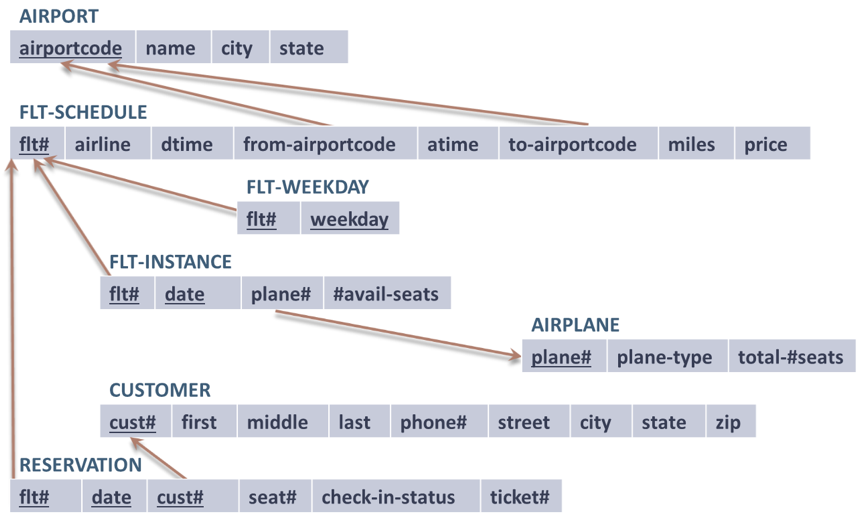
\includegraphics[width=.8\linewidth]{relations.png}
  \caption{Σχεσιακό μοντέλο}
\end{figure}

\subsection{Όψεις}
(Κατασκευάστε χρήσιμες όψεις για τη βάση. Κάθε όψη θα πρέπει να
οριστεί με σχεσιακή άλγεβρα)

Παράδειγμα για τη FlightsDB:

έστω η σχέση:

\begin{itemize}[noitemsep]
\item FLIGHT(flight\_id, airline, fromairport, toairport, price,
  plane\_id)
\item AIRPLANE(plane\_id, plane\_name) 
\end{itemize}

Μια όψη που περιέχει όλες τις αεροπορικές εταιρίες που υπάρχουν στο
σύστημα και τα ονόματα των αεροπλάνων που χρησιμοποιούν είναι η
παρακάτω:

ρAIRLINES(πairline, plane\_name(πairline, plane\_id(FLIGHT)
πplane\_id, plane\_name(AIRPLANE)))



%%% Local Variables:
%%% mode: latex
%%% TeX-master: "main"
%%% End:
